%%%%%%%%%%%%%%%%%%%%%%%%%%%%%%%%%%%%%%%%%%%%%%%%%%%%%%%%%%%%%%%%%%%%%%%%%%%%%
% 26/05/2010
% edited by Bill Lampos
%
% Feel free to use (copy) the structure (latex formatting source code)
% but not the content of this document.
%
%%%%%%%%%%%%%%%%%%%%%%%%%%%%%%%%%%%%%%%%%%%%%%%%%%%%%%%%%%%%%%%%%%%%%%%%%%%%%
\documentclass{beamer}
\usepackage{etex}
\mode<presentation>

\usetheme{Warsaw}
% other themes: AnnArbor, Antibes, Bergen, Berkeley, Berlin, Boadilla, boxes, CambridgeUS, Copenhagen, Darmstadt, default, Dresden, Frankfurt, Goettingen,
% Hannover, Ilmenau, JuanLesPins, Luebeck, Madrid, Maloe, Marburg, Montpellier, PaloAlto, Pittsburg, Rochester, Singapore, Szeged, classic

%\usecolortheme{lily}
% color themes: albatross, beaver, beetle, crane, default, dolphin, dov, fly, lily, orchid, rose, seagull, seahorse, sidebartab, structure, whale, wolverine

%\usefonttheme{serif}
% font themes: default, professionalfonts, serif, structurebold, structureitalicserif, structuresmallcapsserif

% pdf is displayed in full screen mode automatically
%\hypersetup{pdfpagemode=FullScreen}

% define your own colours:
%\definecolor{Red}{rgb}{1,0,0}
%\definecolor{Blue}{rgb}{0,0,1}
%\definecolor{Green}{rgb}{0,1,0}
%\definecolor{magenta}{rgb}{1,0,.6}
%\definecolor{lightblue}{rgb}{0,.5,1}
%\definecolor{lightpurple}{rgb}{.6,.4,1}
%\definecolor{gold}{rgb}{.6,.5,0}
%\definecolor{orange}{rgb}{1,0.4,0}
%\definecolor{hotpink}{rgb}{1,0,0.5}
%\definecolor{newcolor2}{rgb}{.5,.3,.5}
%\definecolor{newcolor}{rgb}{0,.3,1}
%\definecolor{newcolor3}{rgb}{1,0,.35}
%\definecolor{darkgreen1}{rgb}{0, .35, 0}
%\definecolor{darkgreen}{rgb}{0, .6, 0}
%\definecolor{darkred}{rgb}{.75,0,0}

%\xdefinecolor{olive}{cmyk}{0.64,0,0.95,0.4}
%\xdefinecolor{purpleish}{cmyk}{0.75,0.75,0,0}

% \usepackage{beamerinnertheme_______}
% inner themes include circles, default, inmargin, rectangles, rounded

%\usepackage{beamerouterthemesmoothbars}
% outer themes include default, infolines, miniframes, shadow, sidebar, smoothbars, smoothtree, split, tree

%\useoutertheme[subsection=false]{smoothbars}

% to have the same footer on all slides
%\setbeamertemplate{footline}[text line]{xxx xxx xxx}
%\setbeamertemplate{footline}[text line]{} % or empty footer

% include packages
\usepackage{verbatim}

\title{Refactoring 102}
\subtitle{or: How I learned to stop worrying and started to remove code}
\author{Alex Poovathingal}
\institute{Gozefo.com}
\date{\today}

\begin{document}

\frame{
	\titlepage
}

\begin{frame}[fragile]
\frametitle{Introduction}
\begin{center}
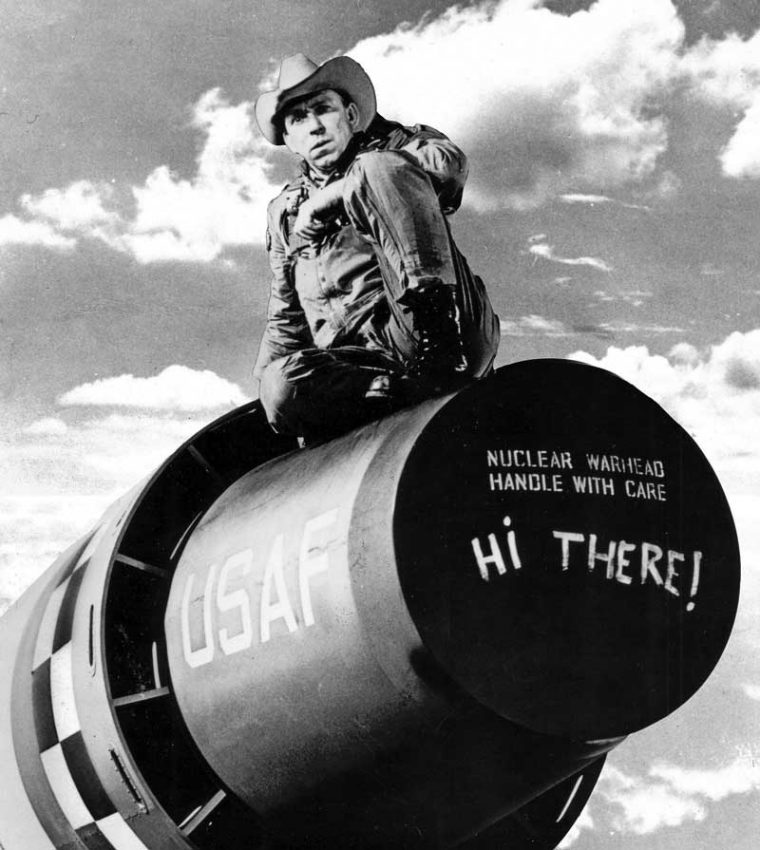
\includegraphics[width=4cm]{resources/strangelove.jpg}
\end{center}
Disclaimer - The author shall not be held liable for any issuesof whatever 
nature which may arise as a result of following these advices.
\end{frame}

\section{Refactoring}
\begin{frame}[fragile]
\frametitle{What is Refactoring}
\begin{itemize}
	\pause
	\item Restructure for the better without changing behaviour
	\pause
	\item Remove code smells
	\pause
	\item Reduce technical debt
	\pause
	\item Without modifying testcases
	\pause
	\item "Leave this world a little better than you found it." - Boy Scout Rule
\end{itemize}
\end{frame}

\begin{frame}[fragile]
\frametitle{When to Refactor and things to keep in mind}
\begin{itemize}
	\item “Don’t stop coding when it starts to work”
	\pause
	\item Yucky code
	\pause
	\item comprehending difficult to understand code should never be the last step
	\pause
	\item "Does this code spark joy" - Marie Kondo
	\pause
	\item Why?? Refactoring is good economics - Is refactoring wasteful rework?
	\pause
	\item Refactor v/s features - do any one at a time - not both
	\pause
	\item Refactor - be ready to throw away code. "Don't be emotionally attached to your code"
	\pause
	\item Workflow - small improvements (always in same direction)
	\pause
	\item File renames or package changes always in different PR and when no one is working on those files
\end{itemize}
\end{frame}

\section{Naming}
\begin{frame}[fragile]
\frametitle{Plurals}
\begin{verbatim}
Integer productsInCart = 2;
\end{verbatim}
\pause
\begin{verbatim}
List<CartProduct> productsInCart = [product1, product2];
\end{verbatim}
\pause
\begin{verbatim}
Better - cartProductCount, cartProductList, 
cartProducts (?)
\end{verbatim}
\pause
\begin{verbatim}
products v/s productList
productNames, productsNames, productsName, productNameList 
\end{verbatim}
\end{frame}

\begin{frame}[fragile]
\frametitle{Proper Names}
\footnotesize
\begin{verbatim}
ProductParts
ProductParts.id and ProductParts.productPartId
\end{verbatim}
\pause
\begin{verbatim}
String productPartId = productPart.getId();
String productPartId = productPart.getProductPartId();
\end{verbatim}
\normalsize
\end{frame}

\begin{frame}[fragile]
\frametitle{Mysql}
\begin{itemize}
	\item Plural table Name (Controversial)
	\item Singular entity
	\item updated\textunderscore on vs updatedOn
	\item Worst case - learn language
\end{itemize}
\end{frame}

\section{Removing Code}
\begin{frame}[fragile]
\frametitle{Removing Code}
\begin{itemize}
	\item Less code, less bugs. No code, ...
	\pause
	\item Unused files, unused functions
	\pause
	\item Unused APIs
\end{itemize}
\end{frame}

\begin{frame}[fragile]
\frametitle{Visual}
\begin{itemize}
	\item Code consistency throughout the project
	\pause
	\item Arguments on each line
	\pause
	\item Easier if condition
	\pause
	\item Readability always
	\pause
	\item Intellij warnings
	\pause
	\item Line length - 150, function length, class length
\end{itemize}
\end{frame}

\section{Workflows}
\begin{frame}[fragile]
\frametitle{Pull Request Etiquettes}
\begin{itemize}
	\item git diff
	\pause
	\item Make life easier for reviewer.
	\pause
	\item Lesser lines - what do each line do
	\pause
	\item Blank lines, format issues, unrelated changes
\end{itemize}
\end{frame}

\begin{frame}[fragile]
\frametitle{Bug fixing Workflow}
\begin{itemize}
	\item Write failing test. Make sure it fails
	\item Make your code change.
	\item Test should pass now
\end{itemize}
\pause
Tests should be
\begin{itemize}
	\item Concise
	\item Readable
	\item Isolated
\end{itemize}
\end{frame}

\section{Unsolicited Advice}
\begin{frame}[fragile]
\frametitle{Unsolicited Advice (Polished Rants)}
\begin{itemize}
	\item Upfront Design v/s evolutionary design
	\pause
	\item If your code is not unit testable, it is bad code
	\pause
	\item Small changes every day take you to big refactoring
	\pause
	\item Compilation errors are good
	\pause
	\item Easy to read, understand, navigate \textgreater\textgreater\textgreater  performance, design pattern, world peace, or any other thing
	\pause
	\item Not everything needs to scale - MOST things doesn't need to scale
	\pause
	\item Code is better than infrastructure
\end{itemize}
\end{frame}

\section*{}
\frame{
    \begin{center}
        \huge
        Any more points?
    \end{center}
}

\end{document}
